\section{Backend}
Backend, neboli serverová část aplikace, našeho projektu slouží primárně k shromažďování a následnému zpracovávání dat. Naše API dále umožňuje bezplatný přístup k těmto datům.
Backend byl vyvinut v Pythonu pomocí knihovny FastApi a pro ukládání dat byla použita databáze PostgreSQL.
Pro odesílání e-mailů byla použita knihovna smtplib a pro komunikaci s platební branou byla použita knihovna stripe. 

Backend může být abstrahována do tří klíčových částí, z nichž každá má specifické úkoly: 
\begin{itemize}
  \item zpřístupnění dat pro Frontend/Developery (pomocí API) 
  \item zajištění komunikace mezi stanicí a databází 
  \item spravování objednávek, objadnané prostřednictvím webové stránky (více popsáno v kapitole \ref{frontend})  
\end{itemize}

\subsection{Zpřístupnění dat}
O zpřístupnění naměřených dat se starají veřejné endpointy, které může kdokoli bezplatně použít, ať už pomocí naší webové stránky, či pomocí našeho API. 
V případě použití těchto endpointů, není potřeba žádná authentifikace a uživateli vrátí vyžádaná data ve formátu JSON. Mezi tyto veřejné endpointy patří:
\begin{itemize}
  \item GET /stations
  \item GET /now/{gps} 
  \item GET /stats/{gps}
\end{itemize}

První endpoint (/stations) jednoduše vrádí GPS souřadnice všech stanice, které jsou v ten moment zapojené.
Za tímto endpointem se schovává vpodstatě jeden SQL dotaz, který z databáze vytáhne všechny aktivní stanice a nakonec funkce vrátí JSON.
\begin{lstlisting}[language=json,firstnumber=1, caption=Příklad požadavku /stations]
{
  "message": "ok",
  "stations": [
    {
      "gps": "50.0993194_14.3596525"
    },
    {
      "gps": "49.7454400_14.0578025"
    }
  ]
}
\end{lstlisting}
Druhý endpoint (/now/{gps}) bere jako parametr GPS souřadnice stanice a podle nich z databáze vytáhne poslední naměřené data dané stanice.
Za tímto endpointem se opět schovává vpodstatě jen jeden SQL dotaz, který z databáze vytáhne poslední naměřené hodnoty konkrétní stanice a nakonec funkce vrátí JSON.
\begin{lstlisting}[language=json,firstnumber=1, caption=Příklad požadavku /now/{gps} ]
{
  "message": "ok",
  "time": "24-12-2022 4:20:00",
  "temperature": -3,
  "humidity": 43,
  "pressure": 100000,
  "wind_speed": 13,
  "wind_direction": "N",
  "rain": 4
}
\end{lstlisting}
Poslední endpoint (/stats/{gps}) má za úkol vracet dlouhodobá zprůměrovaná data v časovém rozmezí, které je určeno pomocí query parametrů,
to znamená "date\_from", "date\_to" a nepovinný parametry "freq", který pevně udává frekvenci průměrování dat. Data se průměrují vzhledem k velikosti časového intervalu.
Data v časovém rozmezí, které je menší než jeden den se průměrují po hodině.
Data v časovém rozmezí, které je větší než jeden den se průměrují po dnech. Data v rozmezí, které je menší než rok se průměrují po týdnech
a pokud je časové rozmezí větší než rok průměr se dělá z dvou týdnů. Pokud je potřeba průměrovat bezohledu na velikost časového rozmezí,
stačí nastavit hodnotu parametru query "freq" a data se budou průměrovat vzhledem k hodnotě "freq" následovně:
\begin{itemize}
  \item 1 -> data se průměrují po 5 minutách
  \item 2 -> data se průměrují po 30 minutách
  \item 3 -> data se průměrují po hodině 
  \item 4 -> data se průměrují po dnech 
  \item 5 -> data se průměrují po týdnech 
  \item 6 -> data se průměrují po dvou týdnech 
  \item 7 -> data se průměrují po čtyřech týdnech 
\end{itemize}
O samotné průměrování hodnot se stará samotná databáze pomocí funkce AVG. Celý časový interval se nejprve rozdělí po časových úseků, které se buď automaticky, nebo podle již zmiňované hodnoty "freq".
Následně se provede SQL dotaz do databáze, který vytáhne zprůměrované hodnoty pro každý časový úsek. Nakonec funkce vrátí tyto hodnoty ve formátu JSON.
\begin{lstlisting}[language=json,firstnumber=1, caption=Příklad požadavku /stats/{gps}]
{
  "message": "ok",
  "data": [
    {
      "time": "1-12-2022 00:00:00",
      "temperature": -3.6,
      "humidity": 41,
      "pressure": 100200,
      "wind_speed": 13,
      "wind_direction": "N",
      "rain": 4,
      "avrage_of": 288
    },
    {
      "time": "2-12-2022 00:00:00",
      "temperature": -2.2,
      "humidity": 49,
      "pressure": 100100,
      "wind_speed": 4,
      "wind_direction": "S",
      "rain": 0,
      "avrage_of": 288
    }
  ]
}
\end{lstlisting}

\subsection{Komunikace se stanicí} \label{komunikace}
Pro komunikaci stanice se serverem stanice využíva dva endpointy:
\begin{itemize}
  \item POST /station/register
  \item POST /station/update
\end{itemize}
V případě prvního endpointu (/station/register) jde primárně o authorizaci stanice, aby data na server nemohl posílat kde kdo. Tento POST požadavek očekává v parametru 
seriové číslo stanice a jeho GPS souřadnice. Backend nejprve ověří, zda seriové číslo odpovídá registrovaným stanicím a pokud ano, tak vytvoří JSON Web Token (dále jen JWT),
kterým se stanice dále prokazuje pří dalších interakcích se serverem. Dále si stanici uloží do databáze do seznamu aktivních stanic.

Druhéh endpoint (/station/update) slouží k přidání naměřených dat stanicí do databáze. V tomto případě server očekává v hlavičce požadavku již zmiňovaný JWT,
podle kterého server pozná o jakou jde stanici a naměřená data, které stanice odeslala ve formátu JSON, zapíše do databáze.

\subsection{Správa objednávek}
Celý náš objednávkový systém slouží k tomu, aby si kdokoli mohl zakoupit naší stanici, čím zajistí, že bude mít možnost měřit počasí kdekoliv bude potřebovat. 
Při vytváření objednávkového systému bylo potřeby nejprve vybrat nějakou platební bránu, která by nám umožnila přijímat platby od zákazníků. V našem případě jsme vybrali platební bránu Stripe.

Pro spravování objednávek backend používá 5 endpointů
\begin{itemize}
  \item POST /payment-webhook
  \item POST /login
  \item GET /orders
  \item GET /order/{id}
  \item POST /update/{id}
\end{itemize}
První endpoint (/payment-webhook) funguje jako webhook\footnote{Webhook je způsob, jakým se automaticky přenášejí data mezi webovými aplikacemi.
Pokud se v jedné aplikaci stane určitá událost, webhook ji zachytí a přenese do druhé aplikace.},
který se zavolá v moment, kdy platební brána vyhodnotí, že objednávka byla zaplacena. V moment kdy se zavolá náš webhook, do databáze se přidá nová objednávka. 
V ten moment se také odešle zákazníkovi e-mail o tom, že objednávka byla přijata. Zárověň příjde e-mail i adminům s upozorněním, že byla vytvořena nová objednávka.

Endpoint (/login) slouží k authorizaci adminů. Admin se pomocí webové stránky může přihlásit a spravovat jednotlivé objednávky.

Endpoitn (/orders) je endpoint, který vrací ID všech objednávek. Tento endpoint je omezen pouze pro adminy.

Endpoitn (/order/{id}) vrací informace konkrétní objednávky.

Poslední endpoint (/update/{id}) slouží opět jen pro adminy a slouží k upravování stavu objednávky.

\subsection{Databáze}
Backend používa již zmiňovanou databázi PostgreSQL, ve které je pět tabulek zobrazených na obrázku č.\ref{model_databaze}.
\begin{figure}[h] 
    \centering
    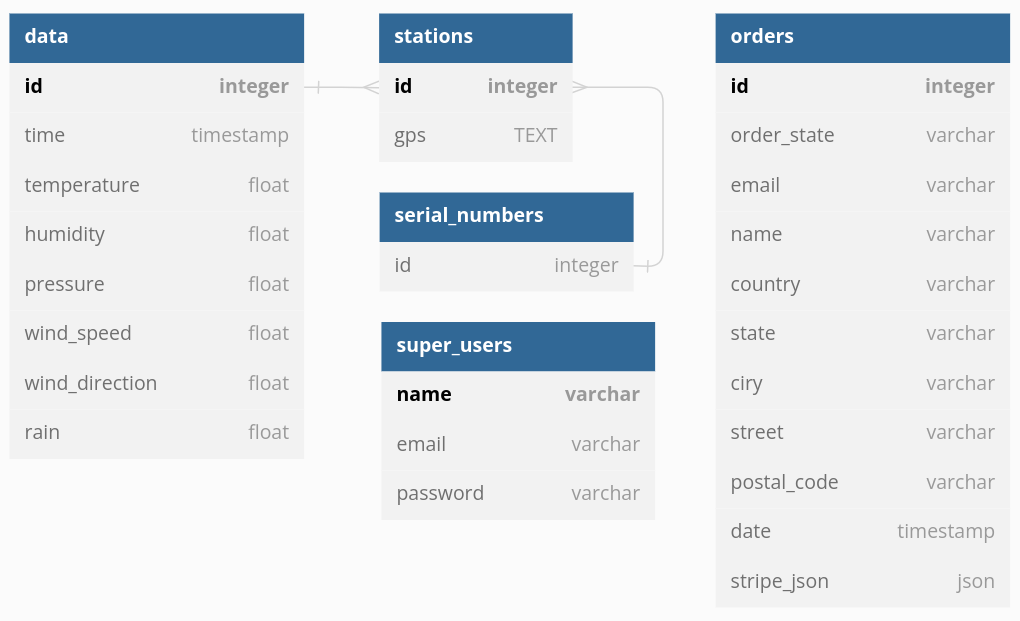
\includegraphics[width=0.8\textwidth]{images/database_diagram.png}
    \caption{Model databáze}
    \label{model_databaze}
\end{figure}
